\documentclass[12pt]{article}
%\renewcommand\normalsize{\fontsize{10pt}{12pt}\selectfont}
\usepackage{graphicx} % Required for inserting images
\usepackage[left=2cm,right=2cm,top=2cm,bottom=1.5cm]{geometry}

\title{HW 5, part 2}
%\author{Dennis Wilkinson}
\date{due Tuesday April 29}

\begin{document}

\setlength{\parindent}{0pt}
\setlength{\parskip}{3mm}

FS1 Wilkinson HW 7, due Monday June 2 

\textbf{1.} In class we discussed how charged objects have electric potential, or voltage, both on them and surrounding them. The potential difference between two points is how much energy it would take to move a positive ``test" charge from one point to the other, divided by the size of the test charge.

\textbf{a.} Which battery is able to cram more charge together on its terminals: a 9V battery or a 1.5 V battery (positive on the cathode, negative on the anode)? Why? The battery does this with a chemical reaction (turning chemical PE into electrical PE). 

\textbf{b.} Consider a metal sphere with radius $R$ and net charge $Q$. We'll define the voltage at its surface as the potential difference between a point on the surface, and a point ``far away". So we need to know the energy required to move a small test charge $q$ from far away onto this sphere. It's $U=\frac{kQq}{R}$, analogous to gravity, but with repelling instead of attracting forces (work required by outside force, not energy converted to KE). Explain why, therefore, the voltage at the surface of the sphere is $\frac{kQ}{R}$. 

\textbf{c.} Calculate the voltage at the surface of a sphere of radius 1 cm that has charge +20 nC (nanocoulombs) using the formula from part (b). Remember, ``voltage" here means the potential difference between the sphere surface and points very far away. The unit is volts, if you use coulombs and meters.

\textbf{d.} If the sphere has double the radius and double the charge, what's $V$ at the surface? Explain conceptually.

\textbf{e.} Now consider the inside of the sphere. It doesn't take any work to move conduction electrons around in there. Explain therefore why $V$ is constant inside the sphere. Graph $V$ as a function of $r$, for $r$ from 0 to ``$\infty$". 

\textit{The main point of this problem was that $V$ is constant in a conductor at equilibrium (e.g., without steady currents).}

\bigskip

\textbf{2.} We modeled a cloud and the ground during a thunderstorm as two sheets of charge. In this problem we calculate the voltage difference between them.

In order to use $V=\frac{kQ}{r}$ here, you'd have to think of all the bits of charge on the cloud and ground as tiny points, and add $\frac{kQ}{r}$ up for each of them. Ugh. Instead, let's go back to the definition: the voltage difference between two points is the amount of energy it would take to move a charge from one place to the other, divided by the amount of charge you're moving. We can calculate this for the cloud/ground.

\textbf{a.} Going back to week 2, an object moved a distance $\Delta x$ against a force $F$ gained potential energy $F\Delta x$. Here, to move a charge $q$, the force is $F=qE$. And we know $E$; it's a constant $\frac{Q}{\epsilon_0 A}$. Say this works out to 200000 N/C for some cloud. And, say this cloud is 800 m above the Earth. Calculate the energy required to move a small charge $q$ from the cloud to the ground, and then, voltage difference between cloud and the ground 

\textbf{b.} Since $V=Ed$ for constant $E$, as you may have found in part a, another unit for electric field is volts/meter. So lightning, or shocks,  happen when the field is more than $3 \times 10^6$ volts per meter (or less in wet air). If an exposed ``hot" wire in your house is at 170 V (max), how close would you have to be to it to get shocked?

\textbf{c.} But wait... the electric field between two sheets of charge is not supposed to depend on the distance we are from either sheet. So as I move my hand towards a doorknob, after scuffling my feet on carpet, how could volts/meter stay constant as my hand gets closer? This is a tricky point (the answer is not only that the ``infinite" sheet approximation is wrong here; it would apply even if you did have infinite sheets).

\bigskip

\textbf{3.} Current in wires. Let's figure out how fast electrons move in a typical household current, like 1.5 amps in a ``14 gauge" copper wire (a wire's \textit{gauge} is related to its width).

\textbf{a.} A current of 1.5 amps means that 1.5 C worth of electrons flow past a given point in the wire every second. How many electrons is this?

\textbf{b.} Imagine the wire as a cylindrical tube whose cross sectional area is $A$. Look up or find the radius or diameter of 14 gauge wire, in millimeters, and calculate $A$ for it (in meters squared). It will be small, in that unit.

The figure below shows how in time $dt$, the electrons in the volume $Av_d dt$ will flow past a given point, if their average drift velocity is $v_d$. Remember that conduction electrons are randomly moving (very fast) in all directions as they bounce around like crazy. But under the influence of voltage, they will drift along the wire, making (very) slow progress as they bounce. 

\textbf{Bonus} (non-calculus). Calculate an electron's average instantaneous (not drift) speed in metal at room temperature, using kinetic theory (it's just one equation we have seen before).

\begin{figure}[h]
    \centering
    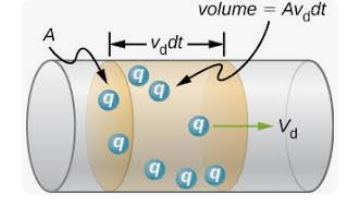
\includegraphics[width=0.5\linewidth]{drift velocity.JPG}
\end{figure}

\textbf{c.} We need to know the number of electrons in this volume. It's the number density of electrons in copper. Look up this number.

\textbf{Another bonus} (non-calculus). Use the density of copper to derive its number density of electrons.

\textbf{d.} Using $dt$ = 1 second, and the results of the problem to this point, figure out the drift velocity of the electrons in an 1.5 A current in 14 gauge copper wire. It should be a fraction of a mm per second.

\textbf{Yet another bonus} (non-calculus). Household current is alternating at a frequency of 60 Hz. This means that 120 times a second, the current switches from one direction to the other; a current of 1.3 A means that 1.3 A is the root-mean-square value of the current as it oscillates. In such a current, roughly far does a typical electron travel in one direction, before reversing direction and going the other way?

\bigskip
\newpage

\textbf{4.} When a wire is connected to the ends of a battery (or similar device which maintains a voltage difference), current flows.

\textbf{a.} The amount of current in the wire increases when the voltage ``across" the battery terminals - meaning the voltage difference between the terminals - increases. Explain why this would be, conceptually.

\textbf{b.} As the electrons are forced to drift one way in the wire, making the current, they undergo more collisions than normal and lose a bit of energy to heat. Explain why more energy would be lost for a skinny wire than a fat wire. What about a long vs a short wire?

\textbf{c.} A simple application here is a toaster heating element, which is simply a long wire (curled up) that gets hot when current flows through it. Consider the following data from testing such an element which has been connected across a voltage $V$ for a while:

\begin{table}[h]
    \centering
    \begin{tabular}{c|c}
         V& I\\
         \hline
         140& 7\\
         120 & 6\\
         100 & 5\\
    \end{tabular}
\end{table}

We define the \textbf{resistance} $R$ by $R=V/I$. What is the resistance for this heating element? Is it constant for different voltages? The unit of resistance is Ohms, $\Omega$; 1$\Omega=1$ volt per amp.

\textbf{d.} When the toaster is first turned on and the element is cold, it's found that for $V=120$, the element draws a current of $I=24$ A. What is the resistance now? Why do you think the resistance is lower when the element is cold than when it is hot? 

\textbf{e.} How much power is the toaster using for $V=120$ when it is hot? (Formula from class.) Where is the power going?  What about when it is first turned on? (This is why in some houses the lights may dim a bit when you turn on a toaster or other appliance). 

\bigskip

\textbf{5*} (worth two questions if you choose it): The potential $\phi$ and the electric field are related by $\vec{\nabla \phi} = \vec{E}$. Consider a metal sphere of radius $R$ with charge $Q$. Show that $\phi(r)=\frac{kQ}{r}$ gives the correct $\vec{E}$ for $r>R$. You can switch to cartesian coordinates for the gradient, or (easier) use spherical coordinates. Repeat for $r<R$; what is $\phi$ here?

  

\end{document}